% MecE 301 1
% FLOW VELOCITY AND FLOW RATE
% You are to evaluate methods of velocity and flow rate measurement with the aim of 
% understanding the characteristics of each device, limitations, and sources of error.
% 1. MEASUREMENT OF AIR VELOCITY - PROCEDURE
% Measurement of flow velocity can be carried out by using many different instruments. In 
% this section of the lab you will investigate the velocity profile of a duct, the effect of 
% probe alignment and then use one flow velocity measurement device to calibrate a 
% second.
% 1.1. EQUIPMENT - Air Velocity Measurement
% The following equipment will be used to measure air velocity:
% • Calibration air jet consisting of an electrically driven centrifugal fan with 
% adjustable inlet damper. The discharge passes through flow straightening tubes in 
% a round pipe, and forms a variable velocity air jet at the pipe exit.
% • Pitot-static tube connected to serve as both stagnation and Pitot-static probes
% • Inclined manometers for stagnation and Pitot-static pressures.
% • Constant temperature hot wire anemometer
% • Metal ruler
% • Mercury barometer
% • Thermometer
% 1.2. Procedure - Measurement of Duct Velocity Profile by Pitot Tube
% Pitot Tube Setup
% A Pitot tube is a device that can measure the local static pressure as well as the stagnation 
% pressure. A schematic of a Pitot tube is shown in Figure 1. The stagnation pressure is the 
% sum of the local pressure as well as the pressure induced by the flow when the fluid is 
% brought to a stop at the end of the tip of the probe. This pressure is a sum of the static 
% and dynamic pressure.
% With the air jet fan off, centre the Pitot static probe by eye in the pipe and align it with 
% the flow direction. Adjust the probe tip so that it is about 10 mm from the pipe exit.
% Adjust the probe so it is aligned with the flow and the protractor is centered at 90°. Move 
% the hot wire anemometer probe out of the flow by sliding it up in the holder. Set the 
% bubble levels on the inclined manometers for proper instrument alignment and adjust the 
% scales to read zero. 
% Measurement of Duct Velocity Profile
% Turn on the fan and adjust the inlet damper plate to produce about an 80% of full scale 
% displacement on the inclined manometers. Using the Pitot-static probe, measure the 
% MecE 301 2
% velocity profile across the duct outlet. You should take at least ten points across the duct 
% to obtain a reasonable representation. Record the data in Table 2.
% Figure 1. A schematic of a Pitot-static tube.
% Effect of Yaw Angle
% The alignment of the Pitot to the flow direction can influence the accuracy of the velocity 
% measurement. This angle, illustrated in Figure 2 is known as the yaw angle of the probe. 
% This section of the lab will investigate the effect of yaw angle on the accuracy of the 
% velocity measurement.
% Adjust the probe so that the tip of the probe is located on the axis of rotation. Measure the 
% effect of yaw angle on both the stagnation and Pitot-static pressures by rotating the probe 
% in its holder. Take at least 5 readings on each side of the correct alignment and record the 
% data in Table 3. 
% Figure 2. The yaw angle of a Pitot tube
% 1.3. Procedure - Calibration of Hot Wire Anemometer
% Calibrate the hot wire anemometer using the Pitot tube as a velocity standard. As 
% previously noted, the velocity profile across the outlet of the discharge pipe is not 
% uniform. Since the two devices cannot be placed in exactly the same location at the same 
% time, the spacing between the probes must be determined. With the fan off, lower the hot 
% wire anemometer probe until the anemometer element is at the same height as the Pitotstatic probe tip. Determine the spacing distance between the hot wire element and the tip 
% of the Pitot static tube using the steel ruler. Zero the anemometer. Turn on the fan and 
% calibrate the anemometer at 10 different flow velocities at the centreline by adjusting the 
% air dampener and record the data in Table 4. The anemometer output voltage may 
% saturate at high velocities (i.e. the voltage will not change with the velocity), so make 
% sure your measurements are below the maximum range of the instrument. At each 
% MecE 301 3
% velocity you will take a reading using the Pitot tube and then move the anemometer to the 
% same point and read the output. 
% Measure the air jet temperature with a thermometer. Read the mercury barometer, 
% applying the appropriate temperature and gravity corrections from the tables provided 
% and record the data in Table 5. 
% 2. AIR FLOW RATE MEASUREMENT - PROCEDURE
% 2.1. EQUIPMENT - Air Flow Rate Measurement
% Air flow rate calibration system consisting of several flow rate meters placed in series 
% along a pipe supplied with compressed air from the building supply. The flow meters and 
% their output devices are:
% • Glass tube rotameter
% • ASME nozzle with 36" U-tube alcohol manometer
% • ASME orifice plate with 60" U-tube alcohol manometer
% • Turbine meter with pulse output and frequency counter
% • Venturi meter with 200 mm H2O Magnehelic gauge and 240 mm water combined 
% inclined/vertical manometer connected in parallel
% • Thermometer
% • D.C. power supply for turbine meter
% 2.2. PROCEDURE - Air Flow Rate Measurement
% Initial system analysis
% Record in Table 6 the internal diameters of the three obstruction meters. Check the zero 
% on the Magnehelic dial gauge and the level bubble and zero setting of the inclinedvertical manometers. Turn on the compressed air supply valve and set the maximum 
% flow rate to 90 or 95% as indicated on the rotameter. The reading from the rotameter is 
% used here only as an indication of the flow rate. The maximum flow rate is limited by the 
% range of the inclined manometers and excess flow will cause the manometers to 
% overflow.
% Divide the available range into ten approximately equal increments, as measured using 
% the rotameter. Measure the output of the six different meters at each of these flow 
% settings, in decreasing order of flow rates and record data in Table 7. Readings should be 
% made simultaneously to allow accurate comparison of the meters. 
% MecE 301 4
% Analysis of calibration data
% For the air flow rate calibration system, assume that the orifice plate is the standard 
% giving the true flow rate within the pipe. 
% Compute the "true" flow rate as measured by the orifice flow meter at each flow rate 
% using Table 1. Recall that the flow rate, Q, of an incompressible fluid through an 
% obstruction meter is:
% (3)
% where A2 is the area of the obstruction, DP is the pressure difference of the obstruction, 
% and r is the density of the fluid. The flow coefficient, K, is;
% (4)
% where C is the discharge coefficient (see below) and b is the ratio of nozzle diameter to 
% pipe diameter.
% Use these computed flow rates to determine the venturi and nozzle discharge coefficients, 
% Cv and Cn. The accepted value (with an uncertainty of 2%) for the nozzle discharge 
% coefficient, Cn, is,
% , for 0.2 ≤ b ≤ 0.8 and 104 ≤ ReD ≤ 107 (5)
% and (6)
% where V is the average velocity of the fluid, µ is the dynamic viscosity, and D is the inner 
% diameter of the pipe.
% The accepted discharge coefficient for a machined venturi is Cv = 0.995 +/- 1% for 
% 50 mm D 250 mm; 0.4 b 0.75; 2x105 ReD 1x106 (ISO standard: 5167-
% 4:2003). Outside the recommend ranges of operation the discharge coefficient may differ 
% by a few percent. 
% The pressure drop in a perfect laminar flow element is linearly proportional to flow rate, 
% Q. Since a real device causes some flow blockage, an additional pressure loss (equivalent 
% to a sudden expansion in a pipe) will add a drop proportional to Q2
% . The expected form 
% of the calibration equation is,
% ΔP = AQ + BQ2 (7)
% where A and B are constants. 
% Fully developed flow is required to ensure accurate measurement with obstruction flow 
% meters. Fully developed flow is typically obtained by using adequate lengths of straight 
% pipe before and after the flow element. Figure 3 shows the recommended minimum 
% lengths of pipe preceding and following orifices, flow nozzles and venturi tubes. The 
% €
% Q = KA2
% 2ΔP
% ρ
% €
% K = C
% 1− β4
% €
% Cn = 0.9965 − 6.53 β
% ReD
% €
% ReD = ρVD
% µ
% €
% ≤
% €
% ≤
% €
% ≤
% €
% ≤
% €
% ≤
% €
% ≤
% MecE 301 5
% diagram that corresponds the closest to the actual piping arrangement for the meter 
% location should be used to determine the required lengths of straight pipe on inlet and 
% outlet (i.e. make some assumptions). These lengths have been determined to hold errors 
% due to piping configurations to less than +/- 0.5% (Fluid Meters: Their Theory and 
% Application, ASME, 1971).
% (a) (b)
% (c) (d)
% Figure 3 Recommended placement of flow meters in different geometries for orifice (a & b) and 
% venturi (c) meter and the effect of valves (d). From Fluid Meters: Their Theory and Application, 
% ASME, 1971. [NOTE: The vertical scale is 'Diameter straight pipe'. This is the number of diameters 
% of pipe you will need before or after the flow meter to ensure the flow is fully developed.]
% MecE 301 6
% Table 1 K values for the lab orifice flow meter 
% (Pipe ID = 74.6 mm, Orifice ID = 27.3 mm, Temperature = 21°C, Patm = 699.0 mmHg)
% DP (inches of alcohol) K, orifice coefficient
% 1.0 0.6095
% 2.0 0.6066
% 3.0 0.6053
% 4.0 0.6045
% 5.0 0.6040
% 6.0 0.6036
% 7.0 0.6033
% 8.0 0.6031
% 9.0 0.6029
% 10.0 0.6028
% 15.0 0.6020
% 20.0 0.6017
% 25.0 0.6015
% 30.0 0.6013
% 35.0 0.6011
% 40.0 0.6011
% 45.0 0.6010
% 50.0 0.6010
% MecE 301 7
% Name:________________________ ID number: ____________________
% Table 2 Air velocity profile at the pipe exit
% Pitot-tube 
% position w.r.t. the 
% pipe centre
% Pitot-tube 
% position (mm)
% Dynamic pressure 
% (mmH2O)
% Stagnation 
% pressure 
% (mmH2O)
% Left
% Centre
% Right
% Table 3 Pitot-tube reading error due to misalignment with the flow direction
% Pitot-tube angle 
% w.r.t. the pipe 
% centreline
% Pitot-tube yaw 
% angle (Deg)
% Dynamic pressure 
% (mmH2O)
% Stagnation 
% pressure 
% (mmH2O)
% Left
% -45
% Centre 0
% Right
% 45
% MecE 301 8
% Table 4 Hot wire anemometer calibration
% Dynamic pressure 
% (mmH2O) Anemometer voltage (V)
% Table 5 Ambient pressure and temperature (used for air density calculation)
% Barometer 
% reading (mmHg) Temperature (o
% C)
% Correction for 
% temperature 
% (mmHg)
% Correction for 
% latitude (mmHg)
% Corrected 
% pressure (mmHg)
% Table 6 Obstruction meter internal diameters
% Nozzle ID (mm) Orifice ID (mm) Venturi ID (mm)
% Table 7 Calibration data from flow rate rig
% Rotameter 
% (%)
% Nozzle 
% (inches of
% alcohol)
% Orifice
% (inches of 
% alcohol)
% Turbine 
% meter
% (Hz)
% Laminar 
% element 
% (mmH2O)
% Venturi Flow
% Temp.
% Magnehelic (°C)
% (cmH2O)
% Inclinometer 
% (mmH2O)
% MecE 301 9
% 4. WORKSHEET
% Collect your data using the Excel file provided on eClass. Most of these calculations are 
% easiest to complete by hand, thus, submit two files: 1) the Excel sheet with your data, and 
% 2) a PDF file showing your calculations and plots. You must show the calculations you 
% used to determine your answers. 
% 1) From Table 5 determine the density of air. (R = 0.287 kJ/(kg K)). (1 mark)
% 2) Determine the maximum velocity (m/s) measured by the pitot-tube in Table 2. (2 
% mark)
% 3) Determine the error in the pitot-tube velocity measurement (m/s) when the yaw 
% angle was -45o relative to the centre value (i.e. 45o to the left). (2 marks).
% 4) Make a plot of the data in Table 4 (1 mark) and determine the sensitivity of the 
% hot-wire anemometer in units of V/(m/s) (1 mark)
% 5) Calculate flow rates measured by the orifice flow meter at each rotameter setting 
% (use K values in Table 1) and show your results in a table. (2 marks)
% 6) Use the maximum computed flow rate to determine the experimentally 
% determined venturi and nozzle discharge coefficients, Cv and Cn. (2 marks) 
% Compare these values to theory. (1 mark)
% 7) Do an uncertainty analysis on the three flowmeters (orifice, machined venturi and 
% nozzle) to determine the expected uncertainty in each meter when the rotameter 
% indicates approximately 50% discharge (3 marks). Assume you can measure the 
% pressure change with a differential pressure sensor with an uncertainty of eDP/DP
% = 2%. Get estimates for the uncertainties in the discharge coefficients from the 
% lecture notes. Assume that the uncertainties in the pipe diameter and obstruction 
% diameter are negligible. Note that the density of the air is a function of 
% temperature and pressure. Assume that you can measure the air pressure with an 
% uncertainty of eP/P = 1% and temperature with an uncertainty of eT/T = 1%. 
% What is the dominant source of uncertainty in each case? (1 mark)
% 8) Make a plot of the turbine meter frequency in Table 7 as function of orifice meter 
% flow rate (1 mark). Calculate the sensitivity of the turbine meter in units of 
% Hz/(m3
% /s) (1 mark).
\DeclareSIUnit\mmwater{mmH_2O}
\DeclareSIUnit\inch{in}
\DeclareSIUnit\inalcohol{inalcohol}
% question 1
\section{}
% Table 5: Ambient pressure and temperature (used for air density calculation)				
% Barometer reading (mmHg)	Temperature (oC)	Correction for temperature (mmHg)	Correction for latitude (mmHg)	Corrected pressure* (mmHg)
% 711	22	2.55	0.4805	708.9305
% * Calculation needed.				
Table \ref{tab:ambient_pressure_and_temperature} shows the ambient pressure and temperature used for air density calculation.

\begin{table}[h]
    \centering
    \caption{Ambient pressure and temperature}
    \label{tab:ambient_pressure_and_temperature}
    \begin{tabular}{p{2cm}p{2cm}p{2cm}p{2cm}p{2cm}}
        \toprule
        Barometer & Temperature & Correction for Temperature & Correction for Latitude & Corrected Pressure \\
        (mmHg) & ($^\circ$C) & (mmHg) & (mmHg) & (mmHg) \\
        \midrule
        711.0 & 22.0 & 2.55 & 0.4805 & 708.9 \\
        \bottomrule
    \end{tabular}
\end{table}

Given that the gas constant for air is $R = \qty{0.287}{\kilo\joule\per\kilogram\per\kelvin}$, the density of air is
\begin{align*}
    PV &= mRT \\
    \implies \rho &= \frac{P}{RT} \\
    &= \frac{708.9/7.501}{0.287 \times (22 + 273.15)} \\
    &= \boxed{\qty{1.12}{\kilogram\per\meter\cubed}}
\end{align*}

% question 2
\section{}
The maximum velocity is given by
\begin{equation}
    v = \sqrt{\frac{2 P_v}{\rho}} \label{eq:velocity from dynamic pressure}
\end{equation}

where $P_v$ is the dynamic pressure and $\rho$ is the density of air. The maximum pressure from 
Table 2 is $P_v = \qty{20.5}{\mmwater}$. From hydrostatic pressure,
\begin{equation*}
    P = h \rho_w g = \qty{1}{\milli\meter} \times \qty{997}{\kilogram\per\meter\cubed} \times \qty{9.81}{\meter\per\second\squared} = \qty{9.78}{\pascal} = \qty{1}{\mmwater}
\end{equation*}
where $\rho_w$ is the density of water \cite{bigg_density_1967}. Thus in (\ref{eq:velocity from dynamic pressure}),
\begin{align*}
    v = \sqrt{\frac{2 \times 20.5 \times 9.78}{1.12}} = \boxed{\qty{19.0}{\meter\per\second}}
\end{align*}

% question 3
\section{}
Similarly, the velocity at a yaw angle of $-45^\circ$ is given by (\ref{eq:velocity from dynamic pressure}) with 
$P_v = \qty{14.5}{\mmwater}$. The velocity is
\begin{align*}
    v = \sqrt{\frac{2 \times 14.5 \times 9.78}{1.12}} = \boxed{\qty{13.6}{\meter\per\second}}
\end{align*}
The error is
\begin{align*}
    err &= 19.0 - 13.6 = \boxed{\qty{5.4}{\meter\per\second}} \\
    \% err &= \frac{19.0 - 13.6}{19.0} \times 100\% = \boxed{28.4\%}
\end{align*}

% question 4
\section{}
\begin{figure}[h]
    \centering
    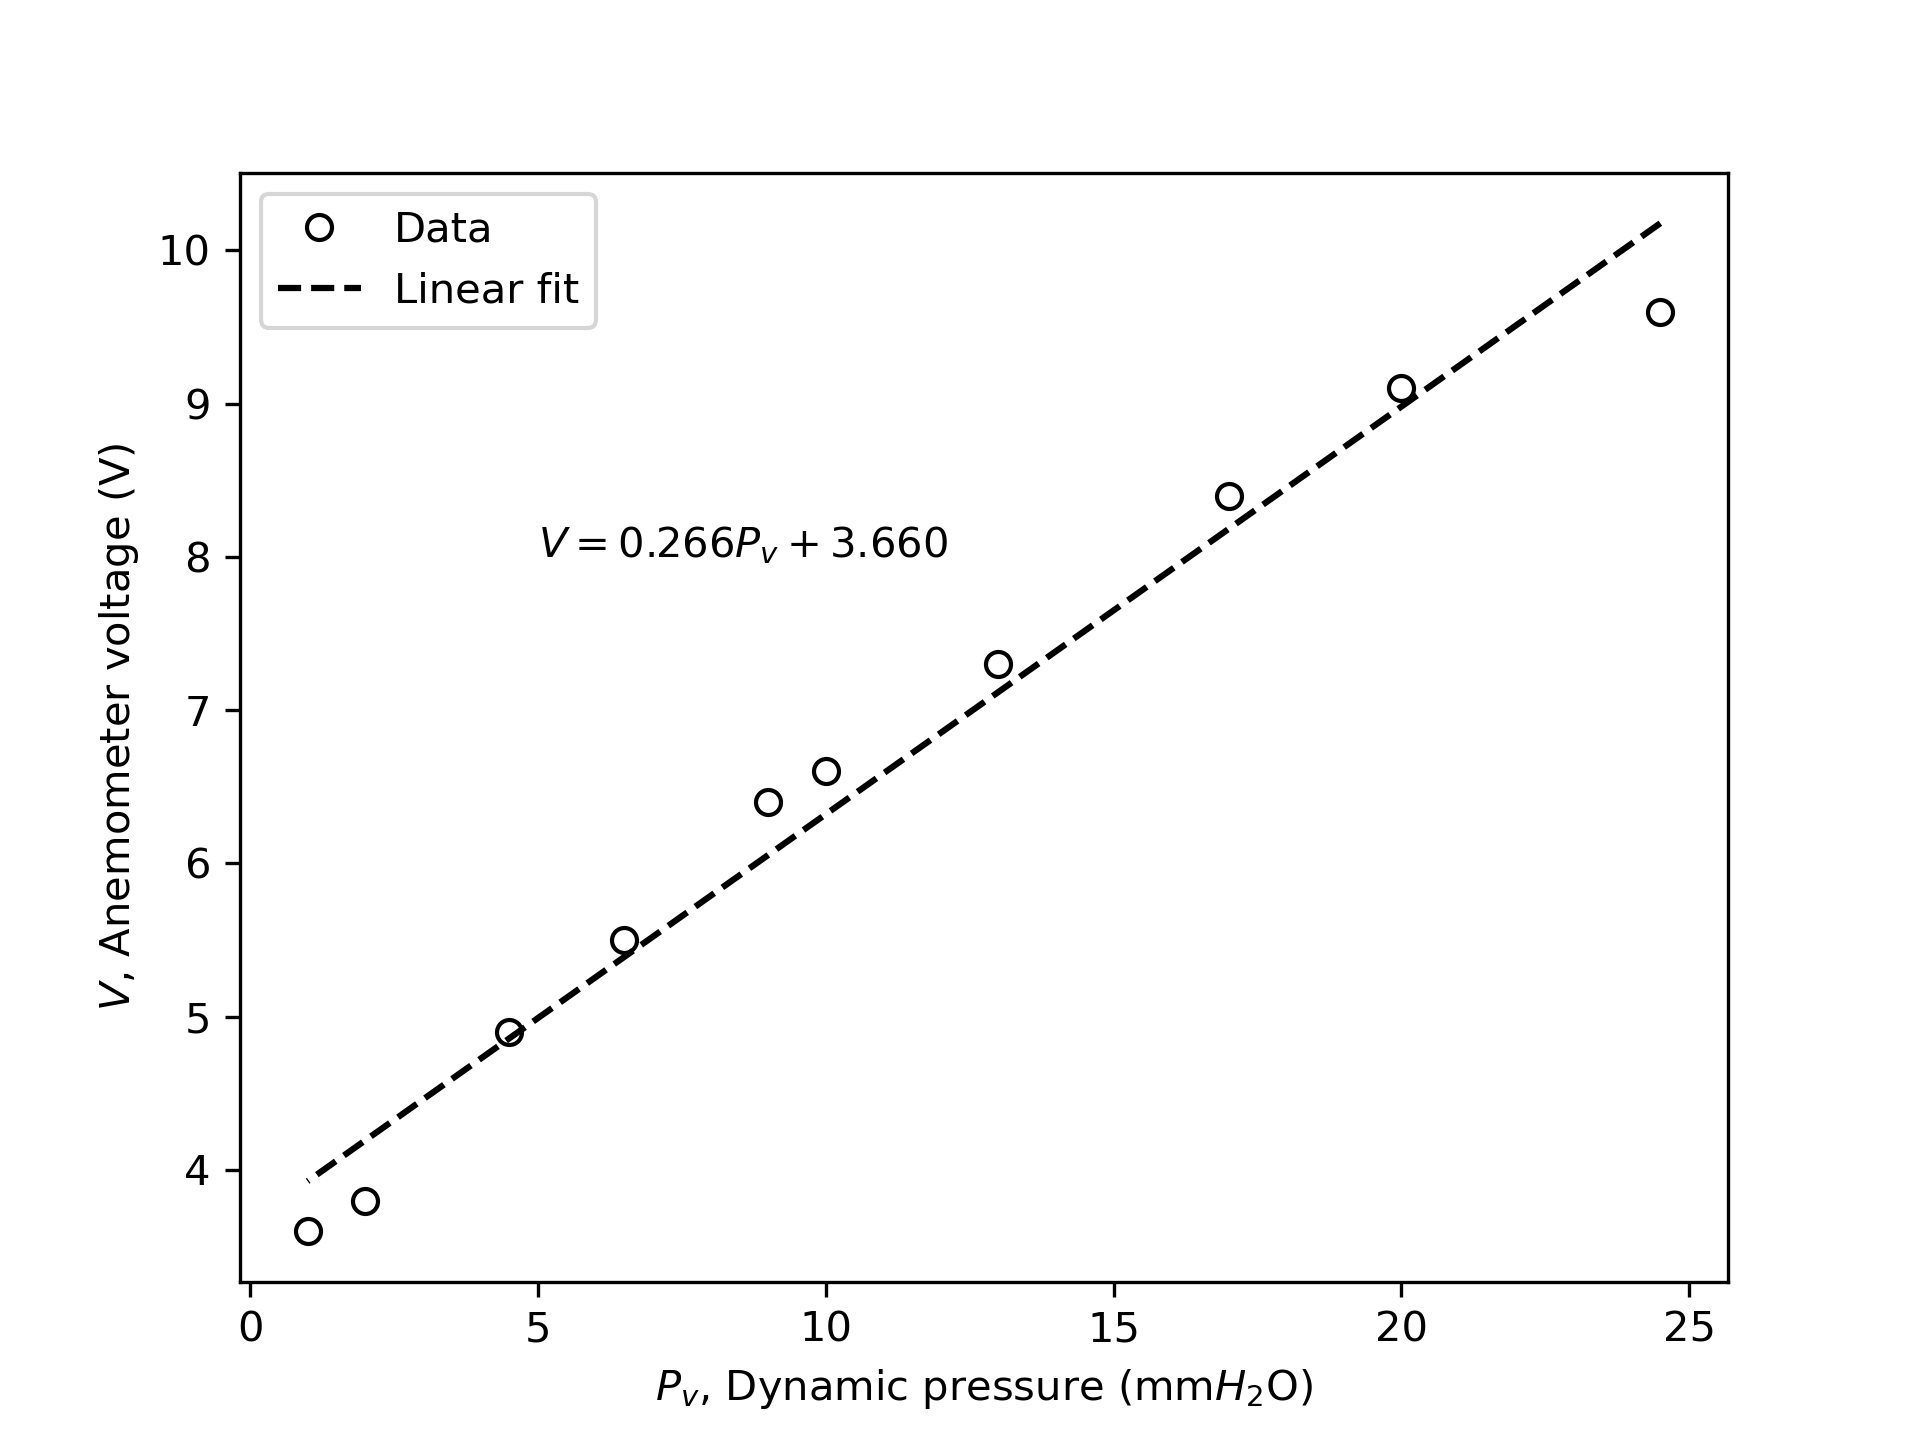
\includegraphics[width=0.8\textwidth]{matplotlib/anemometer_calibration.png}
    \caption{Anemometer voltage response to dynamic pressure}
    \label{fig:anemometer_calibration}
\end{figure}

From the linear regression $y = ax + b$ in Figure \ref{fig:anemometer_calibration}, the sensitivity is
\begin{equation*}
    sensitivity = a = \boxed{\qty{0.27}{\volt\per\meter\per\second}}
\end{equation*}

% question 5
\section{}
The pressure of the orifice is given in the units of inches of alcohol. Converting using $\rho_{alcohol} = \qty{790}{\kilogram\per\meter\cubed}$ 
\cite{ferner_alcohol_2001}.
\begin{align*}
    P_v = \qty{1}{\inalcohol} \times \frac{\qty{1}{\meter}}{\qty{39.37}{\inch}} \times 
    \qty{790}{\kilogram\per\meter\cubed} \times \qty{9.81}{\meter\per\second\squared} = \qty{196.8}{\pascal}
\end{align*}

\begin{table}[h]
    \centering
    \caption{Orifice calibration}
    \label{tab:orifice_calibration}
    \begin{tabular}{p{2cm}p{2cm}p{2cm}p{2cm}}
        \toprule
        $K$ & $A_c$ & $\Delta P$ & $Q$ \\ 
        & (m$^2$) & (Pa) & (m$^3$s$^{-1}$) \\
        \midrule
        0.60116 & 5.15$\times 10^{-4}$ & 1.66$\times 10^3$ & 0.0169 \\
        0.60144 & 5.15$\times 10^{-4}$ & 1.31$\times 10^3$ & 0.0150 \\
        0.60162 & 5.15$\times 10^{-4}$ & 1.08$\times 10^3$ & 0.0136 \\
        0.60186 & 5.15$\times 10^{-4}$ & 822 & 0.0119 \\
        0.60234 & 5.15$\times 10^{-4}$ & 616 & 0.0103 \\
        0.60290 & 5.15$\times 10^{-4}$ & 421 & 0.00852 \\
        0.60348 & 5.15$\times 10^{-4}$ & 313 & 0.00736 \\
        0.60458 & 5.15$\times 10^{-4}$ & 201 & 0.00590 \\
        0.60647 & 5.15$\times 10^{-4}$ & 108 & 0.00434 \\
        0.60950 & 5.15$\times 10^{-4}$ & 48.9 & 0.00294 \\
        \bottomrule
    \end{tabular}
\end{table}

Sample calculations for the first row of Table \ref{tab:orifice_calibration} are shown below.
\begin{align*}
    P_v &= 33.5 \times 196.8 = \qty{6594.48}{\pascal} \\
    A_c &= \frac{\pi}{4} \times \left(27.3/1000\right)^2 = \qty{5.15E-4}{\meter\squared} \\
    K &= \frac{0.6011 - 0.6013}{35-30}(33.5 - 30) + 0.6013 = 0.60116 \\
    Q &= K A_c \sqrt{\frac{2 P_v}{\rho}} = 0.60116 \times 5.15 \times 10^{-4} \times \sqrt{\frac{2 \times 6594.48}{1.12}} 
    = \boxed{\qty{0.0169}{\meter\cubed\per\second}}
\end{align*}
% question 6
\section{}
\FloatBarrier

% Q	Pressure	beta	A_c	C_d	C_d
% Venturi	0.0383	1662.697	0.40616622	0.000721066	0.959657799	0.9965
% Nozzle	0.0383	3208.620	0.343163539	0.000514719	0.974380037	0.977314712
\begin{table}[h]
    \centering
    \caption{Venturi and nozzle discharge coefficients}
    \label{tab:venturi_and_nozzle_discharge_coefficients}
    \begin{tabular}{p{2cm}p{2cm}p{2cm}p{2cm}p{2cm}}
        \toprule
        $Q$ & $P_v$ & $\beta$ & $A_c$ & $C_d$ \\
        (m$^3$s$^{-1}$) & (Pa) & & (m$^2$) & \\
        \midrule
        0.0383 & 1662.7 & 0.4062 & 0.000721 & 0.960 \\
        0.0383 & 3208.6 & 0.3432 & 0.000515 & 0.974 \\
        \bottomrule
    \end{tabular}
\end{table}
For the venturi meter, 
\begin{align*}
    P_v &= 170 \times 9.78 = \qty{1662.7}{\pascal} \\
    \beta &= \frac{d}{D} = \frac{30.3}{74.6} = 0.4062 \\
    A_c &= \frac{\pi}{4} \times \left(30.3/1000\right)^2 = \qty{0.000721}{\meter\squared} \\
    C_d &= \frac{Q_{\text{actual}}\sqrt{1 - \beta^4}}{A_c} \sqrt{\frac{\rho}{2 P_v}} \\
    &= \frac{0.0383 \times \sqrt{1 - 0.4062^4}}{0.000721}\sqrt{\frac{1.12}{2 \times 1662.7}} = \boxed{0.960}
\end{align*}
For the venturi meter theoretical discharge coefficient, $\boxed{C_{d, \text{theory}} = 0.9965}$.

For the nozzle meter,
\begin{align*}
    P_v &= 16.3 \times 196.8 = \qty{3208.6}{\pascal} \\
    \beta &= \frac{d}{D} = \frac{25.63}{74.6} = 0.3432 \\
    A_c &= \frac{\pi}{4} \times \left(25.63/1000\right)^2 = \qty{0.000515}{\meter\squared} \\
    C_d &= \frac{Q_{\text{actual}}\sqrt{1 - \beta^4}}{A_c} \sqrt{\frac{\rho}{2 P_v}} \\
    &= \frac{0.0383 \times \sqrt{1 - 0.3432^4}}{0.000515}\sqrt{\frac{1.12}{2 \times 3208.6}} = \boxed{0.974}
\end{align*}
For the nozzle meter theoretical discharge coefficient, 
\begin{align*}
    V &= \frac{Q}{A_c} = \frac{0.0383}{0.000515} = \qty{8.76}{\meter\per\second} \\
    \text{Re}_D &= \frac{\rho V D}{\mu} = \frac{1.12 \times 8.76 \times 74.6/1000}{1.8347 \times 10^{-5}} = 3.97 \times 10^5 \\
    C_{d, \text{theory}} &= 0.9965 - 6.53 \sqrt{\frac{0.3432}{3.97 \times 10^5}} = \boxed{0.977}
\end{align*}
where $\mu$ is the dynamic viscosity of air at $23^\circ$C \cite{bond_viscosity_1937}.

\textbf{The nozzle is closer to the theory than the venturi meter.}

% question 7
\section{}
Error prop for air density, $\rho$,
\begin{align*}
    \rho &= P^1 R^{-1} T^{-1} \\
    \frac{\delta \rho}{|\rho|} &= \sqrt{\left((1) \frac{\delta P}{|P|}\right)^2 +  \left((-1)\frac{\delta T}{|T|}\right)^2} \\
    &= \sqrt{\left(1\times 0.01\right)^2 + \left((-1)\times 0.01\right)^2} \\
    &= \pm 0.0141
\end{align*}
Error prop for $Q$,
\begin{align*}
    Q &= C_{d}^1 A_{c}^1 (1-\beta^4)^{-1} \sqrt{2}P_{v}^{\frac{1}{2}} \rho^{-\frac{1}{2}} \\
    \frac{\delta Q}{|Q|} &= \sqrt{\left((1) \frac{\delta C_d}{|C_d|}\right)^2 + \left(\left(\frac{1}{2}\right)\frac{\delta P_v}{|P_v|}\right)^2
    + \left(\left(-\frac{1}{2}\right)\frac{\delta \rho}{|\rho|}\right)^2} \\
\end{align*}
For the orifice meter, $\delta C_d/|C_d| = 0.005$, $\delta P_v/|P_v| = 0.01$, and $\delta \rho/|\rho| = 0.0141$. Thus,
\begin{align*}
    \frac{\delta Q}{|Q|} &= \sqrt{\left(0.005\right)^2 + \left(\frac{1}{2}\times 0.01\right)^2 + \left(-\frac{1}{2}\times 0.0141\right)^2} \\
    &= \pm 0.01
\end{align*}
For the venturi meter, $\delta C_d/|C_d| = 0.02$, $\delta P_v/|P_v| = 0.01$, and $\delta \rho/|\rho| = 0.0141$. Thus,
\begin{align*}
    \frac{\delta Q}{|Q|} &= \sqrt{\left(0.02\right)^2 + \left(\frac{1}{2}\times 0.01\right)^2 + \left(-\frac{1}{2}\times 0.0141\right)^2} \\
    &= \pm 0.02
\end{align*}
For the nozzle meter, $\delta C_d/|C_d| = 0.01$, $\delta P_v/|P_v| = 0.01$, and $\delta \rho/|\rho| = 0.0141$. Thus,
\begin{align*}
    \frac{\delta Q}{|Q|} &= \sqrt{\left(0.01\right)^2 + \left(\frac{1}{2}\times 0.01\right)^2 + \left(-\frac{1}{2}\times 0.0141\right)^2} \\
    &= \pm 0.02
\end{align*}

For the orifice meter, the $\rho$ term is the dominant term as
\begin{align*}
    &\left(\left(-\frac{1}{2}\right)\frac{\delta \rho}{|\rho|}\right)^2 > \left(\left(\frac{1}{2}\right)\frac{\delta P_v}{|P_v|}\right)^2 
    = \left(\frac{\delta C_d}{|C_d|}\right)^2 \\
    \iff &\left(\frac{1}{2}\times 0.0141\right)^2 > \left(\frac{1}{2}\times 0.01\right)^2 = \left(0.005\right)^2
\end{align*}
For the venturi, the dominant term is $C_d$ as 
\begin{align*}
    &\left(\frac{\delta C_d}{|C_d|}\right)^2 > \left(\frac{1}{2}\times \frac{\delta \rho}{|\rho|}\right)^2 > \left(\frac{1}{2}\times \frac{\delta P_v}{|P_v|}\right)^2 \\
    \iff &\left(0.02\right)^2 > \left(\frac{1}{2}\times 0.0141\right)^2 > \left(\frac{1}{2}\times 0.01\right)^2
\end{align*}
Lastly, for the nozzle, the dominant term is $C_d$ as
\begin{align*}
    &\left(\frac{\delta C_d}{|C_d|}\right)^2 > \left(\frac{1}{2}\times \frac{\delta \rho}{|\rho|}\right)^2 > \left(\frac{1}{2}\times \frac{\delta P_v}{|P_v|}\right)^2 \\
    \iff &\left(0.01\right)^2 > \left(\frac{1}{2}\times 0.0141\right)^2 > \left(\frac{1}{2}\times 0.01\right)^2
\end{align*}

% question 8
\section{}
\begin{figure}[h]
    \centering
    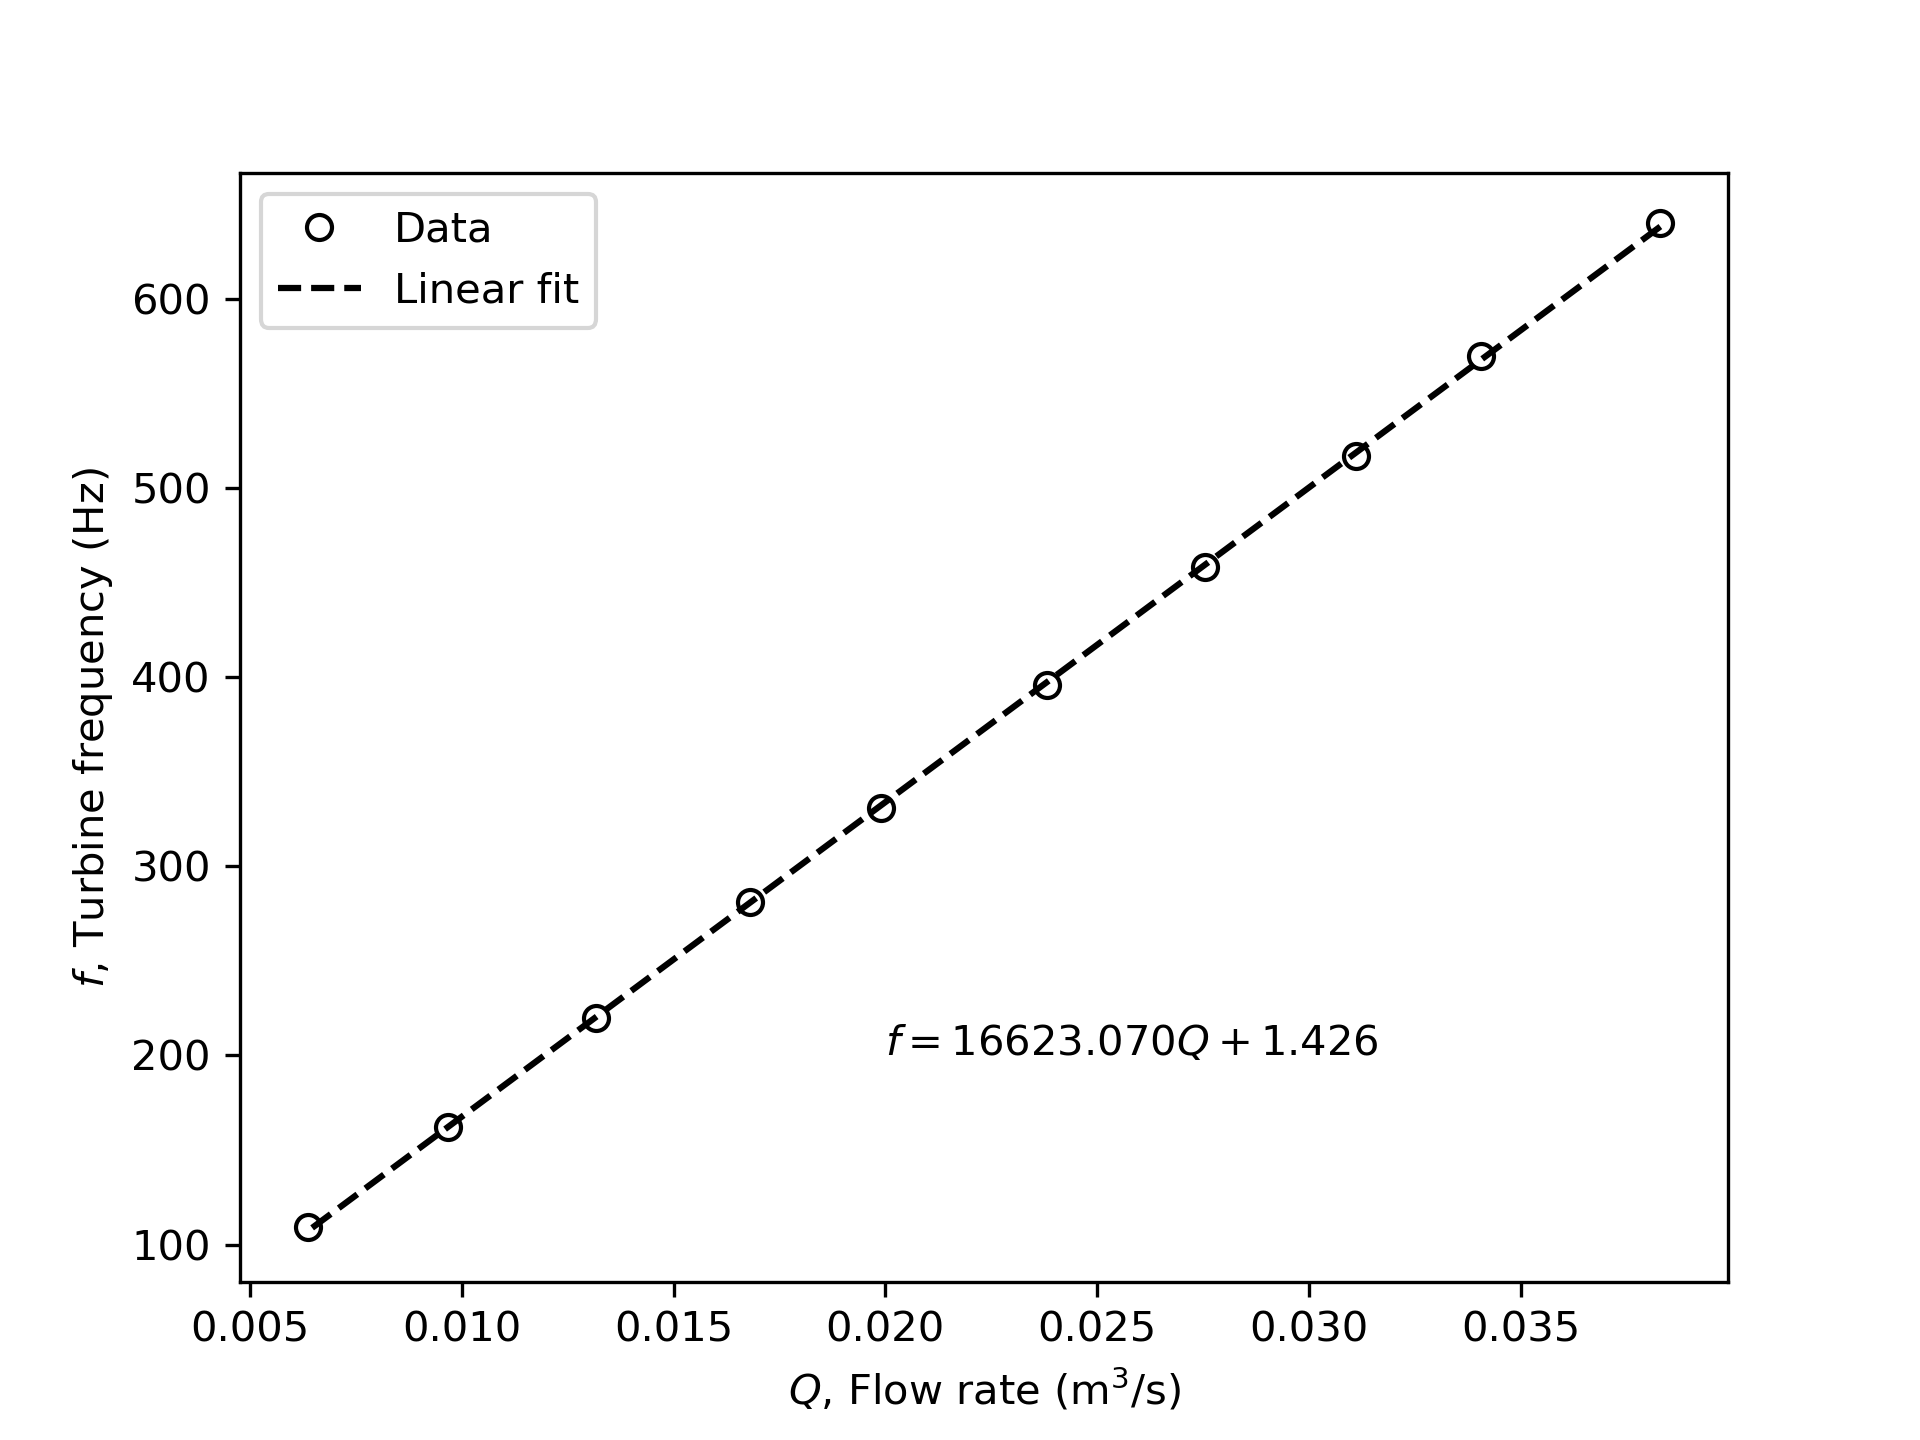
\includegraphics[width=0.8\textwidth]{matplotlib/turbine_calibration.png}
    \caption{Turbine meter frequency response to orifice meter flow rate}
    \label{fig:turbine_meter_calibration}
\end{figure}

From the linear regression $y = ax + b$ in Figure \ref{fig:turbine_meter_calibration}, the sensitivity is
\begin{equation*}
    \boxed{sensitivity = \qty{1.7E4}{\hertz\second\per\meter\cubed}}
\end{equation*}
